\chapter{Korrektur gekrümmte Leinwand}
\label{sec:korrektur gekrümmte leinwand}

\section{Problemursache}
\subsection{Hauptproblem}
Die Leinwand des Fahrsimulators ist nicht flach sondern besitzt eine halbkreisförmige Form. Der Eye Tracker hat keine Einstellmöglichkeit, um eine gekrümmte Leinwand zu berücksichtigen. Dadurch entstehen starke Abweichungen zwischen der vom Eye Tracker geschätzten Blickposition und der realen Blickposition. Abbildung \ref{fig:kruemmungsproblem_1} visualisiert dieses Problem. 



\begin{figure}
	\begin{center}
		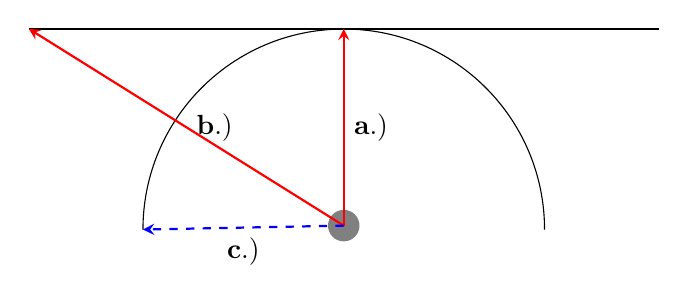
\begin{tikzpicture}
			%\draw [lightgray](0,0) grid (10,10);
			
			
			% Zeichnet die Flache Leinwand
			\draw[thick] (1,9) -- (9,9);
			
			% Zeichnet die linke und rechte Häfte des Halblreises der Leinwand
			\draw (2.45,6.45) arc (180:90:2.546479);
			\draw (7.55,6.45) arc (0:90:2.546479);
			
			% Zeichnet Kreis die Testperson darstellt 
			\fill[gray] (5, 6.5) circle [radius=0.2];
			
			% Zeichnet Pfeil 1 (zeigt direkten Blick nach vorne)
			\draw[thick][-stealth][red] (5,6.5) -- (5,9) node[midway, right, black] {$\mathbf{a.)}$};
			
			% Zeichnet Pfeil 2 (zeigt Blick nach links)
			\draw[thick][-stealth][red] (5,6.5) -- (1,9) node[midway, right, black] {$\mathbf{b.)}$};
			
			% Zeichnet Pfeil 3 (zeigt falsche Anzeige auf Bildschirm)
			\draw[thick][dashed][-stealth][blue] (5,6.5) -- (2.45,6.45) node[midway, below, black] {$\mathbf{c.)}$};
		\end{tikzpicture}
		\caption{Visualisierung der verzerrenden Wirkung einer gekrümmten Leinwand auf die Ergebnisse des Eye Trackers} \label{fig:kruemmungsproblem_1}
	\end{center}
	% Das Label wird gebraucht, um im Text auf diese Abbildung zu referenzieren
\end{figure}

In Abbildung \ref{fig:kruemmungsproblem_1} ist die gekrümmte Leinwand, sowie eine flache Leinwand zu erkennen. Aus Sicht des Eye Trackers existiert nur die flache Leinwand. Ein kleiner grauer Punkt visualisiert die Position der Testperson im Fahrsimulator. Pfeil a.) zeigt direkt von der Testpostion in einem Winkel von 0° auf die Mitte der Leinwand. Es ist zu erkennen, dass es in diesem Punkt keine Abweichung zwischen der flachen Leinwand und der gekrümmten Leinwand gibt. Aus diesem Grund ist zu erwarten, dass der Eye Tracker in diesem Punkt die genausten Ergebnisse liefert. 

Pfeil b.) zeigt ein zweites Szenario. Die Testperson schaut in diesem Fall nach links. Es ist zu erkennen, dass sie mit ihrem Blick die gekrümmte Leinwand auf der linken Seite etwas links von der Mitte trifft. Wenn der Blick der Testperson allerdings imaginär verlängert wird und dadurch auf die imaginäre, flache Leinwand trifft, wird die Abweichung erkennbar. Es ist zu erwarten, dass der Eye Tracker die Blickposition auf den linken Bildschirmrand schätzt, obwohl die reale Blickposition einen gewissen Abstand zum Bildschirmrand besitzt. In einem optimierten System würde der Eye Tracker die Blickposition, welche mit Pfeil b.) dargestellt ist, nur dann schätzen, wenn die Testperson auf den Punkt schaut, welcher mit Pfeil c.) dargestellt ist.


\subsection{Variabilität des Problems}

Es besteht kein gleichbleibender Zusammenhang zwischen der Blickposition auf der flachen Leinwand und der gekrümmten Leinwand. In Abbildung \ref{fig:kruemmungsproblem_2} sind zwei Beispiele zu erkennen. In Beispiel 1 wird der Blick auf die gekrümmte Leinwand mit dem Pfeil a.) dargestellt. Die Transformation auf die flache Leinwand wird mit Pfeil b.) visualisiert. Bei diesem Beispiel schaut die Testperson in einem Winkel $\alpha$ = 90° nach links. Zwischen dem Blick a.) und dem transformierten Blick b.) stellt sich ein Winkel ein. In Beispiel 2 wird nicht an den Bildschirmrand der gekrümmten Leinwand geschaut, sondern in die Mitte. Der Winkel $\beta$ = 45° stellt sich ein. Auch zwischen dem Blick c.) und dem transformierten Blick d.) stellt sich ein Winkel ein. Aus der Abbildung ist zu abzulesen, dass der Winkel zwischen b.) und a.) kleiner ist als der Winkel zwischen c.) und d.). Das zeigt, dass die Transformation zwischen der gekrümmten und der flachen Leinwand nicht konstant ist. Das Problem ist an den Rändern stärker ausgeprägt als in der Nähe der Mitte.

\begin{figure}
	\begin{center}
		\begin{tikzpicture}
			%\draw [lightgray](0,0) grid (10,10);
			
			
			% Zeichnet die Flache Leinwand
			\draw[thick] (1,9.05) -- (9,9.05);
			
			% Zeichnet die linke und rechte Häfte des Halblreises der Leinwand
			\draw (2.45,6.5) arc (180:90:2.546479);
			\draw (7.55,6.5) arc (0:90:2.546479);
			
			% Zeichnet Kreis die Testperson darstellt 
			\fill[gray] (5, 6.5) circle [radius=0.2];
			
			% Zeichnet Pfeil 1 (zeigt direkten Blick nach vorne)
			\draw[thick][black] (5,6.5) -- (5,9.05) node[midway, right, black] {$\mathbf{1.5 m}$} coordinate (direkt);
			
			% Zeichnet Pfeil 2 (zeigt Blick nach links)
			\draw[thick][-stealth][red] (5,6.5) -- (2.45, 6.5) node[midway, below, black] {$\mathbf{a.)}$} coordinate (blick);
			
			%Ursprung zwischen den zwei Pfeilen 
			\coordinate (O) at (5,6.45);
			
			% Shorthandoff muss dazu geschrieben werden, weil es sonst durch das german Language Pack Probleme mit den Anführungszeichen kommt!
			\shorthandoff{"}%
			% Zeichnet einen Winkel zwischen den beiden Pfeilen 
			\pic [draw, <->,
			angle radius=8mm, angle eccentricity=1.2,
			"$\alpha$"] {angle = direkt--O--blick};
			\shorthandon{"}%
			
			% Zeichnet Pfeil 3 (zeigt Transformation zwischen gekrümmter und flacher Leinwand)
			\draw[thick][-stealth][blue] (2.45, 6.5) -- (1, 9.05) node[midway, right, black] {$\mathbf{b.)}$} coordinate;
			
			
			
			% Zeichnet Pfeil 3 (zeigt Blick nach links weiter in Mitte)
			\draw[thick][-stealth][red] (5,6.55) -- (3.22, 8.3) node[midway, left, black] {$\mathbf{c.)}$} coordinate (blick2);
			
			% Zeichnet Pfeil 4 (Transformatio von c.) zu flacher Leinwand)
			\draw[thick][-stealth][blue] (3.22, 8.3) -- (3, 9.05) node[midway, left, black] {$\mathbf{d.)}$} coordinate;
			
			\shorthandoff{"}%
			% Zeichnet einen zweiten Winkel zwischen den beiden weiteren Pfeilen 
			\pic [draw, <->,
			angle radius=12mm, angle eccentricity=1.2,
			"$\beta$"] {angle = direkt--O--blick2};
			\shorthandon{"}%
			
			% Zeichnet Pfeil 3 (zeigt Transformation zwischen gekrümmter und flacher Leinwand)
			\draw[thick][-stealth][blue] (2.45, 6.5) -- (1, 9.05) node[midway, right, black] {$\mathbf{b.)}$} coordinate;
			
		\end{tikzpicture}
		\caption{Visualisierung der nichtlinearen Transformation} \label{fig:kruemmungsproblem_2}
	\end{center}
\end{figure}



\subsection{Problem der Sitzposition}

In den Abbildungen \ref{fig:kruemmungsproblem_1} und \ref{fig:kruemmungsproblem_2} wurde die Sitzposition der Testperson im Fahrsimulator immer im Mittelpunkt der gekrümmten Leinwand angekommen. In der Realität sitzt die Testperson nicht in der Mitte des Halbkreises, sondern näher in Richtung Leinwand. Ein Mensch hat ein Sichtfeld von ca. 200° \cite{lit_website_doccheck_fov}. Würde die Testperson in der Mitte des Halbkreises sitzen, dann würde die Leinwand 180° des Sichtfeldes umfassen. Da die Testperson aber näher an der Leinwand sitzt und somit nicht mehr in der Mitte des Halbkreises, befinden sich die Ränder der Leinwand weiter hinten und das Sichtfeld wird noch weiter ausgereizt. Kopfbewegungen im Eye Tracker sind nicht optimal. Da die Ränder der Leinwand nur durch eine kleine Kopfbewegung in das Sichtfeld rutschen, resultiert daraus eine verringerte Genauigkeit des Eye Trackers in der Nähe der Bildschirmränder.

Eine weitere Abweichung von den Annahmen weiter oben ist die um links verschobene Sitzposition der Testperson im Fahrsimulator. Bisher wurde angenommen, dass die Testperson direkt gegenüber der Mitte der Leinwand sitzt. In der Realität ist sie durch das nachgebaute Fahrzeugcockpit leicht nach links versetzt. Dadurch verhält sich die Transformation von flacher auf gekrümmte Leinwand links anders als rechts. Abbildung \ref{fig:kruemmungsproblem_3} visualisiert diese Einflüsse. 


\begin{figure}
	\begin{center}
		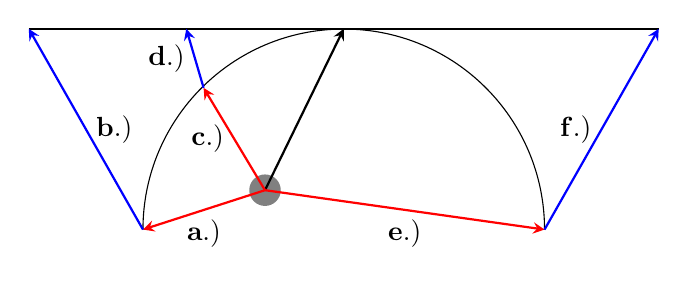
\begin{tikzpicture}
			%\draw [lightgray](0,0) grid (10,10);
			
			
			% Zeichnet die Flache Leinwand
			\draw[thick] (1,9.05) -- (9,9.05);
			
			% Zeichnet die linke und rechte Häfte des Halblreises der Leinwand
			\draw (2.45,6.5) arc (180:90:2.546479);
			\draw (7.55,6.5) arc (0:90:2.546479);
			
			% Zeichnet Kreis die Testperson darstellt 
			\fill[gray] (4, 7) circle [radius=0.2];
			
			% Zeichnet Pfeil 1 (zeigt direkten Blick nach vorne)
			\draw[-stealth][thick][black] (4,7) -- (5,9.05) node[midway, right, black] {$\mathbf{}$} coordinate (direkt);
			
			% Zeichnet Pfeil 2 a.)(zeigt Blick nach links)
			\draw[thick][-stealth][red] (4,7) -- (2.45, 6.5) node[midway, below, black] {$\mathbf{a.)}$} coordinate (blick);
			
			%Ursprung zwischen den zwei Pfeilen 
			\coordinate (O) at (4,7);
			
			
			
			
			% Zeichnet Pfeil 3 b.) (zeigt Transformation zwischen gekrümmter und flacher Leinwand)
			\draw[thick][-stealth][blue] (2.45, 6.5) -- (1, 9.05) node[midway, right, black] {$\mathbf{b.)}$} coordinate (blick_transform);
			
			
			
			% Zeichnet Pfeil 4 c.)(zeigt Blick nach links weiter in Mitte)
			\draw[thick][-stealth][red] (4,7) -- (3.22, 8.3) node[midway, left, black] {$\mathbf{c.)}$} coordinate (blick2);
			
			% Zeichnet Pfeil 5 d.) (Transformatio von c.) zu flacher Leinwand)
			\draw[thick][-stealth][blue] (3.22, 8.3) -- (3, 9.05) node[midway, left, black] {$\mathbf{d.)}$} coordinate (blick2_transform);
			
			
			% Zeichnet Pfeil 6 e.)(zeigt Blick nach rechts)
			\draw[thick][-stealth][red] (4,7) -- (7.55, 6.5) node[midway, below, black] {$\mathbf{e.)}$} coordinate (blick3);
			
			% Zeichnet Pfeil 7 f.) (Transformatio von e.) zu flacher Leinwand)
			\draw[thick][-stealth][blue] (7.55, 6.5) -- (9, 9.05) node[midway, left, black] {$\mathbf{f.)}$} coordinate (blick3_transform);
			
		\end{tikzpicture}
		\caption{Visualisierung der Verschiebung der Sitzposition der Testperson} \label{fig:kruemmungsproblem_3}
	\end{center}
\end{figure}

Es ist zu erkennen, dass in diesem Szenario vor allem zwischen der Blickrichtung c.) und der Transformation d.) kaum Fehler besteht. Durch die Sitzposition weiter links wird dort eine geringere Abweichung zwischen gekrümmter und flacher Leinwand bestehen. Experimente am Fahrsimulator haben diese Annahme bestätigt. Besonders in der Mitte der linken Seite hat der Eye Tracker gut geschätzt. Weiter links und sehr weit rechts wurde die Genauigkeit ohne eine Transformation auf die gekrümmte Leinwand wesentlich schlechter. 



\section{Lösungsansatz}

Wie im Abschnitt davor bereits beschrieben, muss eine Transformation zwischen den beiden Leinwänden durchgeführt werden. Die Richtung der Transformation wird dabei durch die Datengrundlage bestimmt. Die Daten stammen vom Eye Tracker und dieser geht von einer flachen Leinwand aus. Dementsprechend muss die Transformation von der flachen Leinwand auf die gekrümmte Leinwand stattfinden. 
Die Sitzposition und der Blinkwinkel bestimmen, wie die Transformation durchzuführen ist. 

Bei der Transformation ist nur die Horizontale von Relevanz. Vertikale Pixel müssen nicht transformiert werden, weil die Leinwand zwar horizontal gekrümmt ist aber nicht vertikal. Es besteht kein vertikaler Fehler zwischen der flachen und der gekrümmten Leinwand. Zu Zwecken der Nachvollziehbarkeit werden zu Beginn zwei einzelne Pixel betrachtet, welche von der flachen Leinwand auf die gekrümmte Leinwand projiziert werden sollen. Beide Pixel sollen sich auf der linken Hälfte der flachen Leinwand befinden. Abbildung \ref{fig:kruemmungsproblem_4} stellt den resultierenden Fehler bei gegebener Sitzposition und Blickrichtung dar. 



\begin{figure}
	\begin{center}
		\begin{tikzpicture}
			%\draw [lightgray](0,0) grid (10,10);
			
			
			% Zeichnet die Flache Leinwand
			\draw[thick] (1,9.05) -- (9,9.05);
			
			% Zeichnet die linke und rechte Häfte des Halblreises der Leinwand
			\draw (2.45,6.5) arc (180:90:2.546479);
			\draw (7.55,6.5) arc (0:90:2.546479);
			
			% Zeichnet Kreis die Testperson darstellt 
			\fill[gray] (4, 7) circle [radius=0.2];
			
			% Zeichnet Pfeil 1 (zeigt direkten Blick nach vorne)
			\draw[-stealth][thick][black] (4,7) -- (5,9.05) node[midway, right, black] {$\mathbf{a.)}$} coordinate (direkt);
			
			%Ursprung zwischen den zwei Pfeilen 
			\coordinate (O) at (4,7);
			
			% Zeichnet Pfeil 4 c.)(zeigt Blick nach links weiter in Mitte)
			\draw[thick][-stealth][red] (4,7) -- (3.22, 8.3) node[right,yshift=-4pt, black] {$\mathbf{d.)}$} coordinate (blick2);
			
			% Zeichnet Pfeil 5 d.) (Transformatio von c.) zu flacher Leinwand)
			\draw[thick][-stealth][blue] (3.22, 8.3) -- (3, 9.05) node[midway, right, black] {$\mathbf{c.)}$} coordinate (blick2_transform);
			
			
			% Zeichnet Pfeil 3 d.) (Zeigt Pfeil ohne korrigierende Transformation)
			\draw[thick][-stealth][green] (3.95,7) -- (2.7, 9.05) node[midway, left, yshift=12pt,xshift=-6pt, black] {$\mathbf{b.)}$} coordinate (blick_transform);
			
			\shorthandoff{"}%	
			\pic [draw, <->,
			angle radius=8mm, angle eccentricity=1.2,
			"$\alpha$", right] {angle = direkt--O--blick2};
			\shorthandon{"}%
			
			\shorthandoff{"}%
			% Zeichnet den Fehler ein 
			\draw [thick](2.7,9.1) -- (3,9.1)
			node[midway,above , black] {$\mathbf{\Delta F}$};
			\shorthandon{"}%
			
		\end{tikzpicture}
		\caption{Graphische Darstellung des Lösungsansatzes für die Transformation} \label{fig:kruemmungsproblem_4}
	\end{center}
	% Lösungsansatz zur Transformation
\end{figure}

In Abbildung \ref{fig:kruemmungsproblem_4} ist der Vektor von der Sitzposition zur Mitte der gekrümmten Leinwand durch a.) gegeben. Die Testperson schaut bezogen auf die gekrümmte Leinwand in Richtung Pfeil d.). Der Eye Tracker würde jetzt allerdings den Punkt auf welchen Pfeil b.) zeigt erkennen. Dieser würde wiederum mit einem anderen Punkt auf dem Halbkreis korrespondieren. Welcher in der Abbildung nicht dargestellt wird, weil es sonst zu unübersichtlich wird. Wichtig ist, dass die Ausgabe des Eye Trackers so transformiert wird, dass er anstatt den Punkt auf welchen Pfeil b.) zeigt, den Punkt, auf welchen Pfeil c.) zeigt, ausgibt. Es muss also eine Transformation um den Fehler $\Delta$ F stattfinden.


Die Berechnung von $\Delta$F ist ein mathematisches Problem. Durch die nach links verschobene Sitzposition und die fehlenden Längenangaben der einzelnen Pfeile ist die Berechnung recht komplex. Ein alternativer Ansatz wäre eine Funktion, welche grob eine Transformation durchführt und vor Ort feinjustiert wird. In Abbildung \ref{fig:kruemmungsproblem_5} ist zu erkennen, dass bei einem Blick in die Mitte der linken Hälfte der gekrümmten Leinwand, eine leichte Korrektur nach rechts notwendig ist. Schaut man auf den Pfeil c.) aus Abbildung \ref{fig:kruemmungsproblem_5} wird klar, dass auf der rechten Seite der Halbkugel eine Korrektur nach links notwendig ist und diese stärker ausfallen muss, als auf der linken Seite. Aus den vorherigen Abbildungen ist zudem herauszulesen, dass das Problem umso stärker wird, je näher sich der Blick den Rändern der Leinwand annähert. Dabei ist es egal, ob linke Hälfte oder rechte Hälfte. 
Allerdings befindet sich der Punkt, welcher keine Korrektur benötigt, nach wie vor in der Mitte der Leinwand, unabhängig von der Sitzposition der Testperson.

\begin{figure}
	\begin{center}
		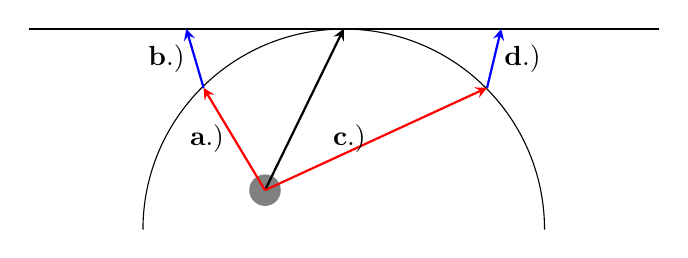
\begin{tikzpicture}
			%\draw [lightgray](0,0) grid (10,10);
			
			
			% Zeichnet die Flache Leinwand
			\draw[thick] (1,9.05) -- (9,9.05);
			
			% Zeichnet die linke und rechte Häfte des Halblreises der Leinwand
			\draw (2.45,6.5) arc (180:90:2.546479);
			\draw (7.55,6.5) arc (0:90:2.546479);
			
			% Zeichnet Kreis die Testperson darstellt 
			\fill[gray] (4, 7) circle [radius=0.2];
			
			% Zeichnet Pfeil 1 (zeigt direkten Blick nach vorne)
			\draw[-stealth][thick][black] (4,7) -- (5,9.05) node[midway, right, black] {$\mathbf{}$} coordinate (direkt);
			
			%Ursprung zwischen den zwei Pfeilen 
			\coordinate (O) at (4,7);
			
			
			
			% Zeichnet Pfeil 4 c.)(zeigt Blick nach links weiter in Mitte)
			\draw[thick][-stealth][red] (4,7) -- (3.22, 8.3) node[midway, left, black] {$\mathbf{a.)}$} coordinate (blick2);
			
			% Zeichnet Pfeil 5 d.) (Transformatio von c.) zu flacher Leinwand)
			\draw[thick][-stealth][blue] (3.22, 8.3) -- (3, 9.05) node[midway, left, black] {$\mathbf{b.)}$} coordinate (blick2_transform);
			
			
			
			% Zeichnet Pfeil 4 c.)(zeigt Blick nach links weiter in Mitte)
			\draw[thick][-stealth][red] (4,7) -- (6.82, 8.3) node[midway, left, black] {$\mathbf{c.)}$} coordinate (blick2);
			
			% Zeichnet Pfeil 5 d.) (Transformatio von c.) zu flacher Leinwand)
			\draw[thick][-stealth][blue] (6.82, 8.3) -- (7, 9.05) node[midway, right, black] {$\mathbf{d.)}$} coordinate (blick2_transform);
			
			
		\end{tikzpicture}
		\caption{Bestimmung der notwendigen Korrektur auf beiden Halbseiten des Halbkreises} \label{fig:kruemmungsproblem_5}
	\end{center}
	% Lösungsansatz zur Transformation
\end{figure}

\subsection{Mathematischer Ansatz e-Funktion}
 

\begin{equation} \label{eq:1}
	k(p) = 
	\begin{cases} 
		e^{c \cdot (w - p)} & \text{für } p \leq w \\
		e^{c \cdot (w - (2w - p))}*k_r & \text{für } p > w
	\end{cases}
\end{equation}

In einem ersten Ansatz wurde eine Korrekturfunktion verwendet, die auf einer e-Funktion basiert. Die Funktion ist dabei abschnittsweise definiert. Je nachdem ob die Testperson auf die linke oder auf die rechte Bildschirmhälfte schaut, wird eine jeweils andere Korrekturfunktion eingesetzt, um den Korrekturwert zu berechnen. Die Abschnittweise Funktion ist in Gleichung \ref{eq:1} zu erkennen.

Dabei ist: 
\begin{center}
	k - Korrektur-Wert\par
	c - Korrektur-Koeffizient (zum Einstellen der Stärke der Korrektur)\par
	w - Bildschirmbreite in Pixel geteilt durch zwei \par
	$k_r$ - Zusätzlicher Korrekturfaktor für rechte Bildschirmhälfte \par
	p - Zu korrigierender Pixel \par
\end{center}

\begin{figure}[h!]
	\begin{center}
		
\includegraphics[scale=0.4]{e_function_param}
		\caption{Sinnvolle Werte für den Korrekturfaktor linke Bildschirmhälfte} \label{fig:imag6}
	\end{center}
\end{figure}

In Abbildung \ref{fig:imag6} ist zu erkennen, wie sich der Korrekturwert bei einer Leinwand mit 4444 Pixeln Breite bezogen auf die jeweiligen Pixel verhält. Der zusätzliche Korrekturfaktor für die rechte Leinwandhälfte $p_{k,r}$ sorgt dafür, dass die Korrektur auf der rechten Hälfte stärker ausgeprägt ist. Das ist notwendig, weil auch der Fehler auf der rechten Bildschirmhälfte stärker auftritt. 

Die Feinabstimmung der Parameter wurde experimentell am Fahrsimulator durchgeführt. Die verwendeten Parameter sind im angehängten Matlab-Skript zu erkennen. 

Mithilfe des Korrekturwertes kann der korrigierte Pixel berechnet werden, wie in Formel \ref{eq:2} zu erkennen ist.  

\begin{equation} \label{eq:2}
	p_{k} =  p \pm k
\end{equation}

Dabei ist: 
\begin{center}
	$p_{k}$ - Korrigierter Pixel \par
	p - Zu korrigierender Pixel \par
	k - Korrektur-Wert\par
\end{center}

Je nachdem ob sich der aktuelle Pixel auf der linken oder rechten Bildschirmhälfte befindet, wird der Korrekturwert auf den zu korrigierenden Pixel addiert oder von diesem subtrahiert. 


Der mathematische Ansatz wurde im Fahrsimulator getestet und es konnten zwar Verbesserungen festgestellt werden, allerdings gab es noch einige Probleme und Optimierungsbedarf. Die Korrektur in der Mitte des Bildschirms ist wesentlich zu schwach. Auch im mittleren Bereich ist sie zu schwach. Zudem sind in Richtung Ränder große Einbußen des Sichtfeldes zu bemängeln. Eine detaillierte Auswertung der Ergebnisse wird hier übersprungen, da schon durch eine erste Beurteilung zu erkennen ist, dass es eine besser geeignete Funktion geben muss. 

\subsection{Limitierung des Sichtbereichs durch Lösungsansatz}

Wie bereits beschrieben erzeugt die Funktion aus dem ersten Ansatz ein verringertes Sichtfeld. Das bedeutet, dass der Eye-Tracker in einem kleineren Bereich als davor funktioniert. Angenommen die Testperson lenkt ihren Blick immer weiter nach links. Ab einem gewissen Punkt erreicht sie den Punkt x=0 auf der imaginären flachen Leinwand. Das entspricht in etwa dem letzten drittel auf der linken Bildschirmhälfte der gekrümmten Leinwand. Ist dieser Punkt erreicht, gibt der Raw-Ouput des Eye Trackers einen Wert von x=0 aus, weil auf einer flachen Leinwand der linken Rand erreicht worden wäre. Bewegt die Testperson ab diesem Punkt den Blick auf der gekrümmten Leinwand noch weiter nach links, dann ändert sich an dem Wert x=0 nichts mehr, weil der Eye-Tracker denkt der Blick der Testperson wären bereits am Rand. Parallel zu diesem Phänomen erreicht der berechnete Korrekturwert am Rand sein Maximum. Angenommen der Korrekturwert würde am Rand eine Wert von 700 Pixel annehmen. Der linke Rand ist auf der flachen Leinwand bei x=0 Pixel. Auf der gekrümmten Leinwand ist dieser Wert allerdings weiter rechts. Die linke Bildschirmhälfte umfasst 2222 Pixel. Der Punkt auf der gekrümmten Leinwand befindet sich ca. am Ende des ersten Drittels. $\frac{1}{3} \cdot 2222 = 740$ Pixel. Wenn dieser Punkt erreicht ist, dann wird auf diese 740 Pixel der Korrekturfaktor von 700 Pixel addiert. Es ergibt sich eine berechnete Position von 740+700 Pixel und somit 1140 Pixel. Schaut die Testperson noch weiter nach links, wird das vom Eye Tracker nicht mehr erfasst, weil die detektierte Blickposition bei der flachen Leinwand weiterhin bei x=0 ist. Auf der gekrümmten Leinwand bleibt die berechnete Blickposition bei x=1140 Pixel hängen. Gleichzeitig bleibt auch der Korrekturwert von 700 Pixel identisch, weswegen eine statische Grenze von 1140 Pixel vom linken Rand entfernt entsteht. Wird der Koeffizient c erhöht, dann wird die Korrekturkurve dadurch steiler. Das wiederum sorgt für einen aggressiveren Korrekturfaktor. Angenommen der aggressivere Korrekturfaktor ist in diesem Beispiel nicht mehr 700 Pixel, sondern 900 Pixel. Die neue statische Grenze liegt jetzt bei 740 Pixel + 900 Pixel = 1640 Pixel vom linken Rand entfernt. Das bedeutet, dass ein höherer Korrekturfaktor c die Korrektur aggressiver macht und gleichzeitig den verwendbaren Bereich des Eye-Trackers einschränkt. Auf der rechten Bildschirmhälfte tritt der Effekt noch stärker auf, da dort noch zusätzlich mit dem Korrekturkoeffizient $k_r$ gerechnet wird. 


Hieraus kann das Fazit gezogen werden: Höherer Korrekturkoeffizient c bedeutet eine aggressivere Korrektur und möglicherweise bessere Ergebnisse. Gleichzeitig wird aber der Sichtbereich, in welchem der Eye Tracker eingesetzt werden kann, verschmälert. Dieses Problem wird auch bei anderen Korrekturfunktion bestehen. 



\subsection{Quadratische-Funktion}

Anstatt einer e-Funktion wird eine quadratische Funktion eingesetzt. Das $k_r$ ist wie bei der e-Funktion nur auf der rechten Bildschirmhälfte anzuwenden. 


\begin{equation} \label{eq:4}
	k(p) = 
	\begin{cases} 
		(c*(w-p))^2 & \text{für } p \leq w \\
		(c*(w-(2*w-x)))^2*k_r & \text{für } p > w
	\end{cases}
\end{equation}

Die Korrektur mit der neuen Funktion wurde im Labor experimentell getestet. Dabei wurde auch Fine-Tuning durchgeführt, um die Funktion so gut es geht an die realen Gegebenheiten anzupassen. Die besten Ergebnisse konnten durch c=0.012 und $k_r=1.5$ erreicht werden. 

\begin{figure}[h!]
	\begin{center}
		
\includegraphics[scale=0.5]{first_correction_function_initialparam}
		\caption{Visualisierung quadratische Korrekturfunktion, Quelle: \cite{lit_software_matlab}} \label{fig:imag8}
	\end{center}
\end{figure}

Wie in Abbildung \ref{fig:imag8} zu erkennen ist, besteht jetzt im Vergleich zur e-Funktion eine stärkere Korrektur in der Nähe der Mitte der Leinwand. An den Rändern ist der Korrekturwert nicht so hoch wie bei der e-Funktion, wodurch der nutzbare Sichtbereich weniger stark eingeschränkt wird. 

Im Fahrsimulator war eine leichte Verbesserung spürbar und es wurde eine Auswertung der Ergebnisse durchgeführt. 

\begin{figure}[h!]
	\begin{center}
		
\includegraphics[scale=0.19]{first_correction_function_results}
		\caption{Gegenüberstellung reale Blickposition und Eye Tracker-Werte: unkalibriert (links), kalibriert (rechts), Quelle: \cite{lit_software_matlab}} \label{fig:imag9}
	\end{center}
\end{figure}

In Abbildung \ref{fig:imag9} sind die Ergebnisse zu erkennen. Auf der x-Achse ist die reale Blickposition in Pixel aufgetragen. Dabei entspricht 0 Pixel dem linken Bildschirmrand und 4444 Pixel dem rechten Bildschirmrand. Die reale Blickposition wurde mithilfe des Mauszeigers ermittelt. Die Testperson hat den Mauszeiger über den Bildschirm bewegt und ihn mit den Augen verfolgt.
Auf der y-Achse ist die vom Eye Tracker geschätzte Blickposition aufgetragen. Diese ist zur Vergleichbarkeit ebenfalls in Pixel angegeben. Für beide Graphen in Abbildung \ref{fig:imag9} werden auf der x-Achse dieselben Werte verwendet. Auf der y-Achse werden beim linken Graphen die Rohdaten des Eye Trackers aufgetragen. Beim rechten Graphen werden die von unserer quadratischen Funktion kalibrierten Werte angezeigt. Im Idealfall sollten die blauen Punkte deckungsgleich mit der hellblauen monoton steigenden Gerade sein. Um zu prüfen, dass unsere Kalibrierung gut funktioniert, sollten die blauen Punkte im rechten Graphen zum einen so nahe wie möglich an der blauen Gerade anliegen und zum anderen bessere Ergebnisse als im linken Graphen erzielt werden. 

Es ist zu erkennen, dass der Sichtbereich auch bei der Verwendung einer quadratischen Korrekturfunktion eingeschränkt wird. Diese Einschränkung konnte allerdings reduziert werden. Bei der e-Funktion war der maximale Korrekturwert auf der linken Bildschirmhälfte k=1300. Bei der abgestimmten, quadratischen Korrekturfunktion liegt das Maximum bei k=700. Es stehen somit auf der linken Bildschirmhälfte 600 Pixel mehr für das Tracking zur Verfügung. Die Auswertung stimmt mit den theoretischen Überlegungen soweit überein, dass bei ca. 2222 Pixel ein Fehler von null vorhanden ist. Das liegt daran, weil die gekrümmte Leinwand und eine äquivalente, imaginäre, gerade Leinwand in der Bildschirmmitte bei 2222 Pixel identisch sind. 
Um die Verbesserungen deutlich zu erkennen, müssen bestimmte Bereiche genauer betrachtet werden: 
-

\begin{figure}[h!]
	\begin{center}
		
\includegraphics[scale=0.19]{first_correction_function_results_zoomed}
		\caption{Gegenüberstellung reale Blickposition und Eye Tracker-Werte im Detail: unkalibriert (links), kalibriert (rechts), Quelle: \cite{lit_software_matlab}} \label{fig:imag10}
	\end{center}
\end{figure}

In Abbildung \ref{fig:imag10} ist ein Detail-Ausschnitt der Ergebnisse der linken Leinwand-Hälfte zu erkennen. Es ist deutlich zu sehen, dass die Werte nach der Kalibrierung näher an der idealen Geraden liegen. Je näher sich die Blickposition dem linken Bildschirmrand näher, umso geringer wird der absolute Fehler. Es ist allerdings auch festzustellen, dass in Richtung Bildschirmmitte weiterhin zu wenig korrigiert wird. Dort ist generell ein geringer Fehler zwischen gekrümmter und gerade Leinwand zu erwarten. Dennoch ist der dort fast so hoch wie in Randnähe. Würde der Parameter c erhöht werden, dann würde der Fehler reduziert werden. Gleichzeitig würde allerdings auch der nutzbare Erfassungsbereich des Eye Trackers reduziert werden. Es bestehen dieselben Probleme wie bei der e-Funktion, nur weniger stark ausgeprägt. 

Eine Funktion 4. Grades scheint auf den ersten Blick sinnvoll. Diese steigt zwar stärker an als eine quadratische Funktion, allerdings besitzt sie in ihrem Ursprung ein Plateau. Dadurch wäre die Korrektur im Bereich der Bildschirmmitte definitiv nicht ausreichend. 


\subsection{V-Funktion mit abgeflachtem Beginn und Ende}

Nach den Experimenten im Fahrsimulator wurde aus den daraus gewonnen Erfahrungen eine Funktion gesucht, welche in der Bildschirmmitte einen Korrekturwert von null ausgibt. Die Funktion sollte einen Korrekturfaktor ausgeben, welcher sich relativ zum Abstand zu der Bildschirmmitte erhöht. Dabei sollte dieser Anstieg bereits unmittelbar um die Bildschirmmitte hoch sein, damit der Fehler dort bereits ausreichend verringert wird. An den Rändern soll sie allerdings nicht zu sehr ansteigen, da sonst der nutzbare Sichtbereich reduziert werden würde. Als Kurvendiagramm sollte die Funktion wie ein V aussehen, dessen Tiefpunkt auf der x-Achse bei der Bildschirmmitte, also bei 2222 Pixeln liegt. In Richtung der Ränder sollte die Steigung der Funktion kleiner werden, damit der nutzbare Sichtbereich des Eye Trackers nicht zu sehr eingeschränkt wird. Dieser sollte im Idealfall größer sein, als bei der quadratischen Funktion. 

Damit die Steigung stufenlos angepasst werden kann, wurde eine Variable p dafür verwendet. Damit keine negativen Werte herauskommen, muss mithilfe des Betrags sichergestellt werden, dass innerhalb der Basis keine negativen Werte vorkommen. Damit die V-Funktion ihren Tiefpunkt in der Bildschirmmitte hat, muss sie um die Bildschirmmitte nach rechts verschoben werden:

\begin{equation} \label{eq:5}
	k=|x-w|^p
\end{equation}

Zusätzlich wird der Faktor c eingeführt, welcher ähnlich wie p die Steigung relativ zum Abstand zur Bildschirmmitte beeinflusst. Allerdings nicht ganz so aggressiv wie p. Ein Parameter d wurde eingeführt, um ein Grund-Offset zu erzeugen, welches bei der Feinabstimmung evtl. nützlich sein könnte. 

\begin{equation} \label{eq:6}
	k=(c*|(x-w)|+d)^p
\end{equation}

Damit sich die Ränder der Funktion gegen einen bestimmten Wert annähern, muss eine Dämpfung in die Funktion eingebaut werden. Diese wird durch eine e-Funktion realisiert. Dadurch ist eine schnelle Annäherung an den Grenzwert sichergestellt. Die vollständige Korrekturfaktor-Funktion ist in Gleichung \ref{eq:7} aufgeführt. Es ist zu beachten, dass es beim Ansatz mit der v-Funktion unterschiedliche Parameter für die linke und rechte Seite der Bildschirmhälfte gibt. Diese sind mit einem herab gestelltem l bzw. r gekennzeichnet. Die zugewiesenen numerischen Werte sind im angehängten Matlab Skript aufgeführt.

\begin{equation} \label{eq:7}
	k(p) = 
	\begin{cases} 
		(c_l*|(w-x)|+d_l)^{p_l}*(1-e^{-g_l*(|w-x|)}) & \text{für } p \leq w \\
		(c_r*|(w-(2*w-x))|+d_r)^{p_r}*(1-e^{-g_r*(|w-(2*w-x)|)}) & \text{für } p > w
	\end{cases}
\end{equation}



\begin{figure}[h!]
	\begin{center}
		
\includegraphics[scale=0.4]{second_correction_function_param}
		\caption{Korrekturfunktion: linke Bildschirmhälfte (links), rechte Bildschirmhälfte (rechts), Quelle: \cite{lit_software_matlab}} \label{fig:imag11}
	\end{center}
\end{figure}


Die graphische Darstellung der Korrekturfunktion ist in Abbildung \ref{fig:imag11} zu erkennen. Die optimalen Parameter wurden im Fahrsimulator experimentell bestimmt und werden für die Darstellung des Graphen verwendet. Wie in der Abbildung zu erkennen ist, unterschieden sich die Parameter zwischen linker und rechter Leinwandhälfte. Auf der rechten Hälfte muss stärker korrigiert werden. Hier ist die Veränderung der Steigung ab einem gewissen Punkt gut zu erkennen. 

Die Auswertung der Ergebnisse erfolgt im nächsten Abschnitt. 